\documentclass[12pt]{book}
\usepackage{geometry}                % See geometry.pdf to learn the layout options. There are lots.
\geometry{letterpaper}                   % ... or a4paper or a5paper or ... 
%\geometry{landscape}                % Activate for for rotated page geometry
%\usepackage[parfill]{parskip}    % Activate to begin paragraphs with an empty line rather than an indent
\usepackage{graphicx}
\usepackage{makeidx}
\usepackage{url}
\usepackage{tikz}
\usetikzlibrary{shapes,arrows}

\makeindex

\title{OpenLCB / NMRAnet S-9.7 DevKit Manual}
%\author{The Author}
%\date{}                                           % Activate to display a given date or no date

\begin{document}
\maketitle

\tableofcontents

\chapter{What's all this in the box?}

Here's what you'll find in the box, and a short description of each to help you get started:
\begin{itemize}
\item 3 x Railstars Io V1.0 boards
\item 1 x TCH Technology OpenLCB USB/CAN Interface board
\item 1 x ButtonLED8 v1.0 board
\item TODO cables
\item TODO potentially useful odds and ends
\end{itemize}

The three Railstars Io boards are the heart of TODO. Each board is designed to connect to various features of your layout, and communicate to each other via the included CAT5 cables.

The TODO ButtonLED8 is a tool to help you quickly get the most from the Railstars Io.

The TCH Technology OpenLCB USB/CAN Interface permits you to expand your layout's capabilities by providing a USB interface to connect your home computer.

\chapter{Basic Concepts of OpenLCB / NMRAnet S-9.7}

TODO What is it?

\section{Producer-Consumer model}
\index{producer-consumer model}

\chapter{Connecting the Railstars Io boards}

\begin{figure}[htbp]
\begin{center}
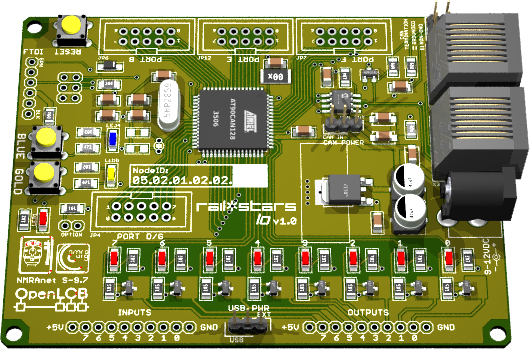
\includegraphics[width=6in]{images/RailstarsIo.png}
\caption{Railstars Io (color may vary)}
\label{Io}
\end{center}
\end{figure}


Railstars Io is an OpenLCB node that provides a set of 16 producers connected to 8 inputs and 16 consumers connected to 8 outputs. The inputs can be used with buttons and switches on a fascia panel, or with existing accessories on your layout such as block detectors or turnout feedback units. The outputs can be used directly to control bulbs or LEDs on your layout, or connected to existing accessories on your layout such as turnout controllers or signal decoders.

\section{Initial Setup}

To use Railstars Io, you will first need to solder the appropriate terminals to the input and output banks. You can solder wires directly to the holes in the circuit board, or solder in the included pin headers or screw terminals. If you are unsure which to use, the screw terminals are the most flexible, and will serve most purposes.

\begin{figure}[htbp]
\begin{center}
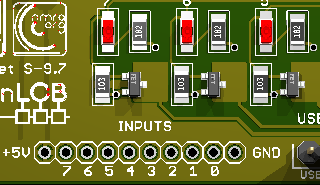
\includegraphics[width=3in]{images/IoInputEmpty.png}
\caption{Railstars Io input bank as shipped}
\label{bareinput}
\end{center}
\end{figure}

\begin{figure}[htbp]
\begin{center}
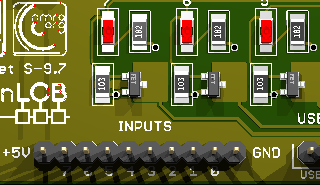
\includegraphics[width=3in]{images/IoInputPinheader.png}
\caption{Railstars Io input bank with pin headers soldered in place}
\label{pinheader}
\end{center}
\end{figure}

\begin{figure}[htbp]
\begin{center}
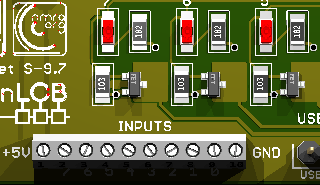
\includegraphics[width=3in]{images/IoInputsWithScrewTerminal.png}
\caption{Railstars Io input bank with screw terminals soldered in place}
\label{screwterminal}
\end{center}
\end{figure}

\section{Connecting to NMRAnet bus}

Connecting Io to your OpenLCB network is simple. Use a CAT5 cable to connect Io to another node in your network.

\index{NMRAnet!termination}Notice that OpenLCB networks must be arranged as a linear string or nodes, and that the two nodes at the end of the network (and only those two nodes) must be terminated. To terminate a node, set the termination jumpers on Io. To remove termination from a node, remove the termination jumpers.

TODO FIGURE OF TERMINATION JUMPERS

\section{Providing power}

Railstars Io can be powered in one of three ways: From an external power supply, via the NMRAnet bus, or via a USB connection to a PC.

\subsection{Powering with an external supply}
\label{externalpower}
\index{Railstars Io!power, power adapter}

You may power Railstars Io using an external power supply that provides a 2.1mm center-positive plug, and between 9 and 12V DC at 500mA or more of current. Ensure that the ``USBPWR'' jumper is set to ``EXT'', as per Figure \ref{EXTPWR}

\begin{figure}[htbp]
\begin{center}
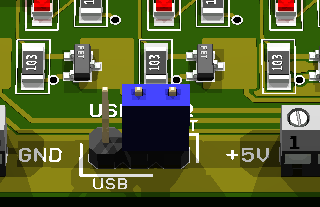
\includegraphics[width=3in]{images/IoUSBPowerEXT.png}
\caption{USBPWR jumper set to external power}
\label{EXTPWR}
\end{center}
\end{figure}

\subsection{Powering via USB}
\index{Railstars Io!power, USB}

Using the included USB cable, you can power Railstars Io via the USB interface. To do so set the ``USBPWR'' jumper is set to ``USB'', as per Figure \ref{USBPWR}, and then plug the USB cable into the FTDI header, following the instructions in \S\ref{FTDI}.

\begin{figure}[htbp]
\begin{center}
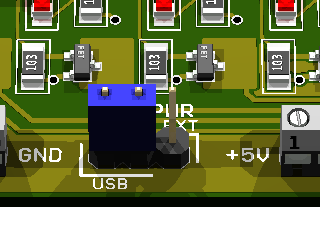
\includegraphics[width=3in]{images/IoUSBPowerUSB.png}
\caption{USBPWR jumper set to USB power}
\label{USBPWR}
\end{center}
\end{figure}

\subsection{Powering via the NMRAnet bus}
\index{Railstars Io!power, NMRAnet from@power, from NMRAnet}
\index{NMRAnet!bus power}

The NMRAnet bus can provide a small amount of power to individual boards. To configure Railstars Io to draw power from the NMRAnet bus, set the ``USBPWR'' jumper to ``EXT'', as per Figure \ref{EXTPWR} above, and then set the ``CAN POWER'' jumper to ``CAN IN'', as per Figure \ref{CANIN}.

\begin{figure}[htbp]
\begin{center}
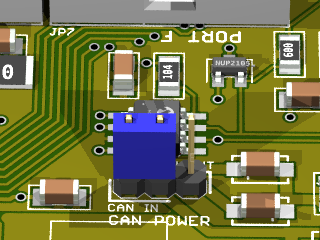
\includegraphics[width=3in]{images/IoCANPowerIn.png}
\caption{CAN POWER jumper set to draw power from the NMRAnet bus}
\label{CANIN}
\end{center}
\end{figure}

Note that drawing power from the NMRAnet bus requires that at least one other node be configured to provide power to the NMRAnet bus.

\subsection{Providing power to the NMRAnet bus}
\index{Railstars Io!power, NMRAnet to@power, to NMRAnet}
\index{NMRAnet!bus power}

A Railstars Io node that is configured to use an external power supply can optionally be configured to provide power to the NMRAnet bus. In this case, a power adapter capable of providing 750mA--1,000mA is suggested. Configure the board as per \S\ref{externalpower}, and then set the ``CAN POWER'' jumper to ``CAN OUT'', as per Figure \ref{CANOUT}.

\begin{figure}[htbp]
\begin{center}
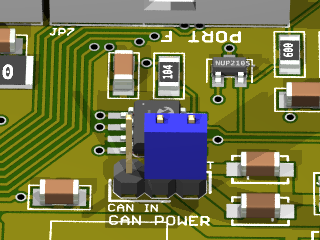
\includegraphics[width=3in]{images/IoCANPowerOut.png}
\caption{CAN POWER jumper set to provide power to the NMRAnet bus}
\label{CANOUT}
\end{center}
\end{figure}

Note: If the Railstars Io will neither draw power from nor provide power to the NMRAnet bus, please remove the ``CAN POWER'' jumper entirely.

\section{Usage Example: ButtonLED8 v1.0}

TODO image of screw terminals and ButtonLED8

The included ButtonLED8 board is a great way to quickly attach a set of inputs to Io. To connect the board, TODO.

Once connected, you can use the buttons on the ButtonLED8 board as inputs; each button press triggers the production of an event, as does each button release. By default, Railstars Io is pre-loaded with a useful configuration for use with ButtonLED8, in that each button will trigger a corresponding output; that is, pressing button 1 will cause the LED wired to output 1 to light.

\section{Usage Example: Fascia panel}

Railstars Io can be used to interface a fascia panel or control panel to your layout. Simply wire the panel switches to the Io inputs, and the panel indicators to the Io outputs as indicated below. By default, Railstars Io is pre-loaded with a useful configuration for fascia panels, in that each input will trigger the corresponding output; that is, pressing a button wired to input 1 will cause a bulb or LED wired to output 1 to light.

\subsection{Wiring inputs to switches}

Inputs should be wired to short to ground. An open circuit on an input is read as ``off'', and shorting the input to ground is read as ``on''. (It is safe to apply 5V to the inputs, although Io cannot distinguish between an open circuit and +5V on an input line).

Normally-open pushbuttons should be wired as per Figure \ref{pushbutton}, with one leg to the desired input, and the other to ground. In this configuration, a depressed button will be read as ``on''.

\begin{figure}[htbp]
\begin{center}
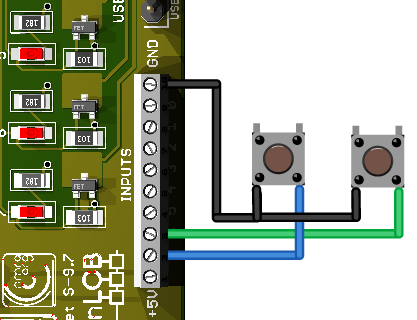
\includegraphics[width=3in]{images/Inputs-pushbutton.png}
\caption{Wiring pushbutton switches to Io inputs}
\label{pushbutton}
\end{center}
\end{figure}

DPDT switches should be wired as per Figure \ref{DPDT}, with the center pin wired to the desired input, one pin wired to ground, and the other left unconnected. In this configuration, moving the toggle towards the wired pin is read as ``on'', and towards the other as ``off''.

\begin{figure}[htbp]
\begin{center}
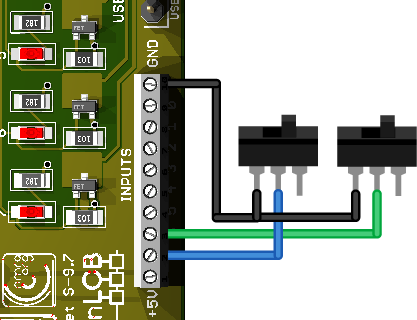
\includegraphics[width=3in]{images/Inputs-DPDT.png}
\caption{Wiring DPDT toggle switches to Io inputs}
\label{DPDT}
\end{center}
\end{figure}


\subsection{Wiring outputs to indicators}

The outputs on Io toggle between open circuit, and shorted to ground. Thus, devices to be controlled should be wired to the +5V and the output line, as per Figure \ref{indicators}. LEDs will require a current-limiting resistor (about 470 ohms will suffice), and their polarity must be carefully observed, with the long pin (anode) wired to the +5V terminal, and the short pin (cathode) wired to the desired output terminal. Incandescent bulbs must be of the 5V variety, but do not require a current-limiting resistor.

\begin{figure}[htbp]
\begin{center}
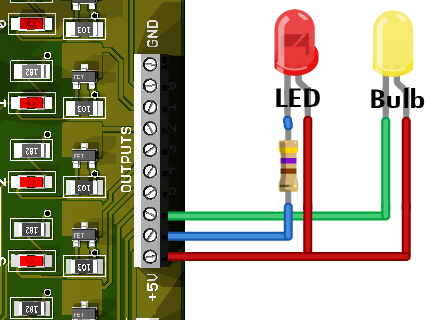
\includegraphics[width=3in]{images/Outputs-indicator.png}
\caption{Wiring LEDs and bulbs to Io output}
\label{indicators}
\end{center}
\end{figure}

\section{Usage Example: Digitrax DS64 Quad Stationary Decoder}

TODO image of screw terminals and DS64

\section{Usage Example: NCE TODO}

\chapter{Configuring Railstars Io}

Out of the box, each Railstars Io produces and consumes the same set of events, so that triggering Input 1 on any Io board will cause LED 1 to light on all connected Io boards. It is easy to configure Io to produce more complex producer-consumer schemes. There are two ways: Using the on-board Blue/Gold interface, or with a PC via a USB connection, which will be covered in the next chapter.

\section{The Blue/Gold Interface}

TODO image of B/G interface

The Blue/Gold interface is a simple way to configure the behavior of Io. The interface consists of two buttons, called Blue and Gold, and two corresponding LEDs. The buttons are used to navigate the configuration options, and the LEDs are used to indicate the state of configuration.

\section{Teaching and Learning}

The basic concept behind configuring any OpenLCB is \textit{teaching}. The process of teaching selects an event associated with one producer or consumer, and assigns it to another producer or consumer. The first consumer or producer must be set up to  "teach", and the second producer or consumer must be set up to "learn". In this way, you can create associations between a producer and a consumer, or mirror a producer to another producer, or a consumer to another consumer.

Configuration is thus a two-step process. First, select the consumer or producer to learn. Second, select the consumer or producer to teach. And that's it!

\section{First Time Setup, and Hard Reset}

Before you begin teaching or learning with Io, you will probably want to perform a Hard Reset. A Hard Reset completely disconnects all producers and consumers on Io from all other nodes on the OpenLCB network. A Hard Reset is like a fresh start, where you can begin anew.

To perform a Hard Reset, press and hold both the Blue and the Gold buttons simultaneously for about 10 seconds; the Blue and Gold LEDs will begin to blink, warning you that you are about to perform a Hard Reset. Continue holding both buttons until the flashing stops. The Hard Reset is complete.

\section{Setting up Learning}

The first step in configuring a new behavior is to select the producer or consumer that will be learning. We begin by pressing the Blue button once. This tells Io to enter Learn Mode. The Blue LED begins to blink, to indicate that Learn Mode has been entered.

The next step depends on whether you want to configure an input or an output for learning.

You can cancel Learn Mode at any time by pressing both Blue and Gold simultaneously. Both the Blue and Gold LEDs will extinguish to indicate that you have left Learn Mode.

\subsection{Configuring an Output for Learning}

Each output has two states: On and off. There are therefore 16 consumers, one for each possible output state. 

Press the Blue button to select Output 0: On. You will observe that the LED for output 0 comes on (and any device attached to the output is triggered). Press the Blue button a second time to select Output 0: Off. The LED for output 0 now flashes to indicate the selection. Press the Blue button a third time to move to Output 1: On, and a fourth time to move to Output 1: Off. Pressing Blue will cycle through all of the outputs/output state combinations in this way.

TODO figure showing LED turning on.

When you have reached the output and output state that you wish to configure for learning, press the Gold Button. The Gold LED will TODO, indicating that the selected output has been configured for learning. You are now ready to set up teaching.

\subsection{Configuring an Input for Learning}

Each input has two states: On and off. There are therefore 16 producers, one for each possible input state.

TODO figure showing connected button and the LED coming on.

To configure an input, you must use an input device connected to the input directly, such as a push-button or toggle switch. Press the push-button or toggle the toggle switch to select that input as "on". Notice that the corresponding output LED will light up to indicate the selection (and that any device attached to the input will also come on; you can safely disregard that action, as we are selecting inputs). To select that input as "off", press the button or toggle the switch a second time. The corresponding LED will now flash. To cancel the selection, press the button or toggle the switch a third time; the corresponding LED will extinguish.

When you have selected the input and input state that you wish to configure for learning, press the Gold Button. The Gold LED will TODO, indicating that the selected input has been configured for learning. You are now ready to set up teaching.

\section{Setting up Teaching}

The second step in configuring a new behavior is to select the producer or consumer that will be teaching. We begin by pressing the Gold button once. This tells Io to enter Teach Mode. The Gold LED begins to TODO, to indicate that Teach Mode has been entered.

You can cancel Teach Mode at any time by pressing both Blue and Gold simultaneously. Both the Blue and Gold LEDs will extinguish to indicate that you have left Teach Mode.

Once you have entered Teach Mode, Outputs and Inputs are selected just as with Learn Mode.

\subsection{Configuring an Output for Teaching}

Each output has two states: On and off. There are therefore 16 consumers, one for each possible output state. 

Press the Blue button to select Output 0: On. You will observe that the LED for output 0 comes on (and any device attached to the output is triggered). Press the Blue button a second time to select Output 0: Off. The LED for output 0 now flashes to indicate the selection. Press the Blue button a third time to move to Output 1: On, and a fourth time to move to Output 1: Off. Pressing Blue will cycle through all of the outputs/output state combinations in this way.

TODO figure showing LED turning on.

When you have reached the output and output state that you wish to configure for teaching, press the Gold Button. The Gold LED will TODO, indicating that the selected output has been configured for teaching. The association has been created, and you are done!

\subsection{Configuring an Input for Teaching}

Each input has two states: On and off. There are therefore 16 producers, one for each possible input state.

TODO figure showing connected button and the LED coming on.

To configure an input, you must use an input device connected to the input directly, such as a push-button or toggle switch. Press the push-button or toggle the toggle switch to select that input as "on". Notice that the corresponding output LED will light up to indicate the selection (and that any device attached to the input will also come on; you can safely disregard that action, as we are selecting inputs). To select that input as "off", press the button or toggle the switch a second time. The corresponding LED will now flash. To cancel the selection, press the button or toggle the switch a third time; the corresponding LED will extinguish.

When you have selected the input and input state that you wish to configure for teaching, press the Gold Button. The Gold LED will TODO, indicating that the selected input has been configured for teaching.  The association has been created, and you are done!

\section{An Example: Associating a Button with an LED}

Scenario: You have two Io boards, Io 1 and Io 2. You wish to associate a switch on Io 1, Input 2 with an LED on Io 2, Output 5 such that flipping the switch up illuminates the LED, and flipping the switch down extinguishes the LED.

\textit{\textbf{Step 1}: Set up Learning for LED On.} On Io 2, press the Blue button to enter Learn Mode. Now, press Blue 11 times to select Output 5: On. Press Gold to mark Output 5: On for learning.

\textit{\textbf{Step 2}: Set up Teaching for Switch Up.} On Io 1, press the Gold button to enter Teach Mode. Now, Move the switch up (if down; if already up, move the switch down, then up) to select that switch. Press the Gold button to teach the association.

\textit{\textbf{Step 3}: Set up Learning for LED off.}. On Io 2, press the Blue button to enter Learn Mode. Now press Blue 12 times to select Output 5: Off. Press Gold to mark Output 5: Off for learning.

\textit{\textbf{Step 4}: Set up Teaching for Switch Up.} On Io 1, press the Gold button to enter Teach Mode. Now, Move the switch up (if down; if already up, move the switch down, then up) to select that switch, and toggle it a second time to select the "off" state. Press the Gold button to teach the association.

Now, test the association. Move the switch up and down, and observe the behavior of the LED. If the LED does not respond as expected, you have probably executed one of the above steps incorrectly, and it so you might simply try the process again. You should not have to perform a Hard Reset, unless things get very out of hand.

\section{An Example: Duplicating a Fascia Panel Button}

Scenario: You have two Io boards, Io 1 and Io 2. Io 1 is already set up to control a fascia panel, and you would like Io 2 to control an identical fascia panel on the other side of the layout. We begin by mirroring the behavior on the push-button attached to Input 0 on both boards; the process is identical for each of the remaining inputs and outputs between the boards.

\textit{\textbf{Step 1}: Set up Learning for Button Down.} On Io 2, press the Blue button to enter Learn Mode. Now, press the push-button once to select it as "down". Press the Gold button to mark that button for learning.

\textit{\textbf{Step 2}: Set up Teaching for Button Down.} On Io 1, press the Gold button to enter Teach Mode. Now, press the push-button once to select it as "down". Press the Gold button to teach the association.

\textit{\textbf{Step 3}: Set up Learning for Button Up.}. On Io 2, press the Blue button to enter Learn Mode. Now, press the push-button twice to select it as "up". Press the Gold button to mark that button for learning.

\textit{\textbf{Step 4}:  Set up Teaching for Button Down.} On Io 1, press the Gold button to enter Teach Mode. Now, press the push-button twice to select it as "up". Press the Gold button to teach the association.

Now, test the association. The push-button on Io 2 should now trigger exactly the same behaviors as the push-button on Io 1. If the layout does not respond as expected, you have probably executed one of the above steps incorrectly, and it so you might simply try the process again. You should not have to perform a Hard Reset, unless things get very out of hand.

\section{Blue/Gold Flow Chart}

%http://www.texample.net/tikz/examples/simple-flow-chart/

\chapter{Using the TCH Technology OpenLCB USB/CAN Interface to connect your PC}

TODO image of USB interface

\chapter{Advanced Topic: Writing custom firmware for Railstars Io}

\section{Connecting the USB adapter}
\label{FTDI}


%%%%%%%%%%%%%%%%%%%%
%end matters

\printindex

\newpage
Figures \ref{DPDT}, \ref{pushbutton}, TODO were created with Fritzing. \url{http://fritzing.org/}

Railstars\texttrademark and Io\texttrademark are trademarks of Railstars Limited. TCH Technology\texttrademark is a trademark of Timothy C. Hatch. NMRA\texttrademark, is a trademark of, and NMRAnet\textregistered and the NMRAnet logo are registered trademarks of the National Model Railroading Association.

TODO Digitrax, NCE

\end{document}  